\documentclass[final]{beamer} % beamer 3.10: do NOT use option hyperref={pdfpagelabels=false} !
\mode<presentation> {  %% check http://www-i6.informatik.rwth-aachen.de/~dreuw/latexbeamerposter.php for examples
  \usetheme{Lankton}    %% you should define your own theme e.g. for big headlines using your own logos 
  \newcommand{\footleft}{}
  \newcommand{\footright}{}
}
\usepackage[english]{babel}
\usepackage[latin1]{inputenc}
\usepackage{amsmath,amsthm, amssymb, latexsym}
\usefonttheme[onlymath]{serif}
\boldmath
\usepackage[orientation=portrait,size=a1,scale=1.4,debug]{beamerposter}                       % e.g. for DIN-A0 poster
\usepackage{tikz}
\usetikzlibrary{shapes.arrows,chains,positioning,automata,trees,calc}
\usetikzlibrary{patterns}
\usetikzlibrary{decorations.pathmorphing,decorations.markings}

\input ../macros.tex
\input ../figures.tex
\input std-macros.tex

\title[NaturalLI]{Natural Logic for Common Sense Reasoning}
\author[Gabor Angeli]{Gabor Angeli}
\institute[Stanford]{Stanford Natural Language Processing}
\date{April 30, 2015}

\newlength{\columnheight}
\setlength{\columnheight}{694mm}

\begin{document}

\begin{frame}{} 
\begin{columns}

\begin{column}{.49\textwidth}
  \begin{beamercolorbox}[center,wd=\textwidth]{postercolumn}
    \begin{minipage}[T]{.95\textwidth}  % tweaks the width, makes a new \textwidth
      \parbox[t][\columnheight]{\textwidth}{% must be some better way to set the the height, width and textwidth simultaneously
        %%%%%%%%%%%%%%%%%%%
% INTRO
%%%%%%%%%%%%%%%%%%%
\begin{frame}{Motivation: Knowledge Base Completion}
\begin{center}
\begin{tabular}{cccc}
  \begin{tabular}{c}
    \h{Unstructured Text} \\
    \\
    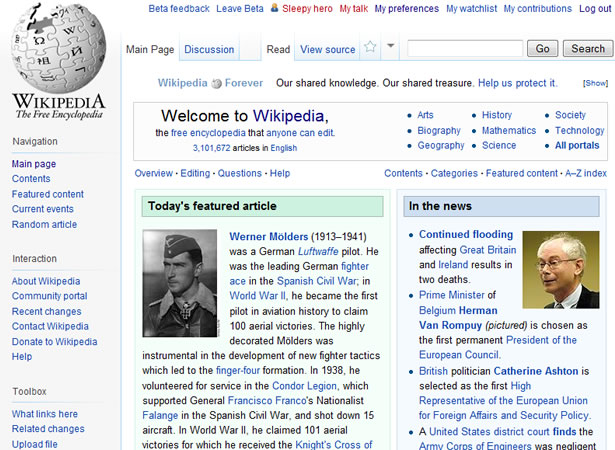
\includegraphics[width=2cm]{../img/wiki.jpg} \\
    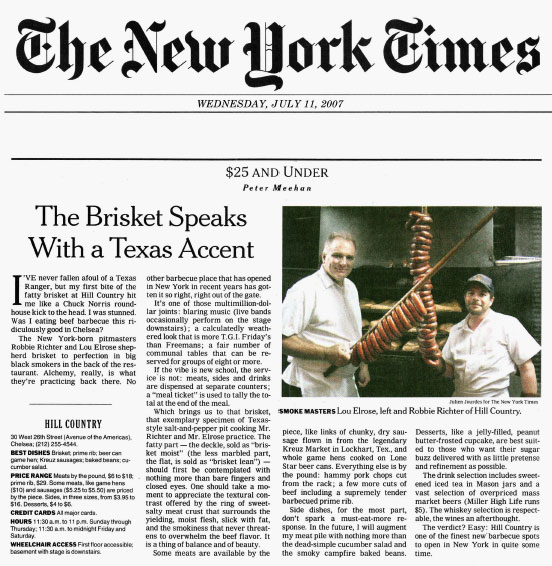
\includegraphics[width=2cm]{../img/nyt.jpg} \\
    
\includegraphics[width=2cm]{../img/blog.jpg}
  \end{tabular} &

  \Huge{$\Rightarrow$} &
  
  \begin{tabular}{c}
  \h{Structured Knowledge Base} \\
  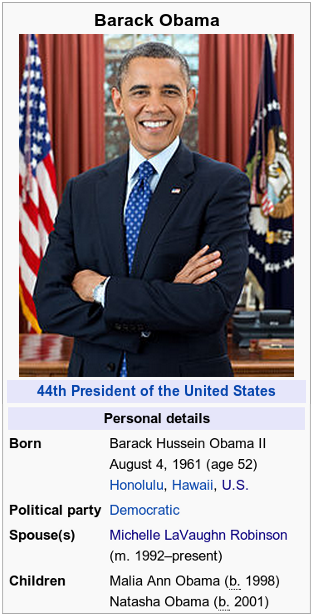
\includegraphics[width=2.75cm]{../img/obama-infobox.png}
  \end{tabular}
\end{tabular}
\end{center}
\end{frame}


%%%%%%%%%%%%%%%%%%%
% MOTIVATION
%%%%%%%%%%%%%%%%%%%
\def\title{Motivation: Question Answering}
\begin{frame}{\title}
\begin{center}
  
\includegraphics[width=7cm]{../img/google-chris-manning-origin.png}
\end{center}
\end{frame}

\begin{frame}[noframenumbering]{\title}
\vspace{-1cm}
\begin{center}
  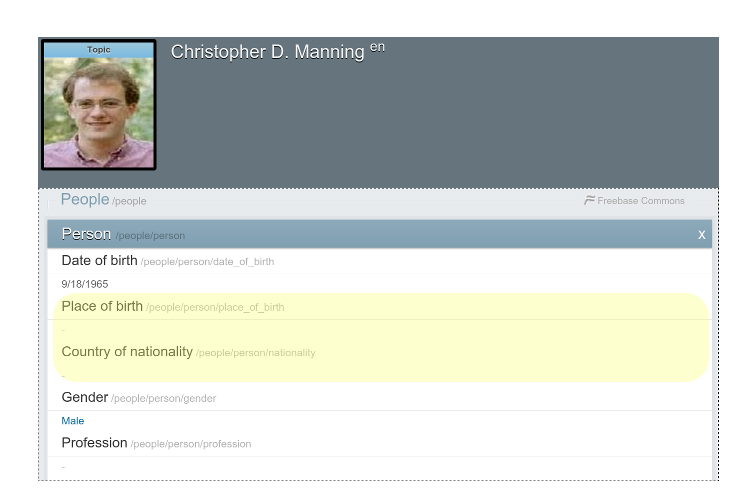
\includegraphics[width=10.5cm]{../img/chris-freebase.png}
\end{center}
\end{frame}

\begin{frame}[noframenumbering]{\title}
\begin{center}
  \begin{tabular}{l}
  
\includegraphics[width=12cm]{../img/chris-website-header.png} \\
  
\includegraphics[width=9cm]{../img/chris-bio.png}
  \end{tabular}
\end{center}
\end{frame}

\begin{frame}[noframenumbering]{\title}
\begin{center}
  \fbox{
\includegraphics[width=7cm]{../img/google-chris-manning-origin-answer.png}}
\end{center}
\end{frame}

        %%%%%%%%%%%%%%%%%%% 
% Natural Logic
%%%%%%%%%%%%%%%%%%%
\begin{frame}{Natural Logic}
\begin{center}
\hh{If I mutate a sentence in this way, do I preserve its truth?}
\end{center}
\vspace{1em}
\pause

\hh{Logic over natural language}
\begin{itemize}
\item \textit{Instantaneous} semantic parsing!
\item Plays nice with lexical methods (ongoing work).
\end{itemize}
\vspace{1ex}
\pause

\hh{Tractable}
\begin{itemize}
\item Polynomial time entailment checking (e.g., MacCartney and Manning 2009).
\end{itemize}
\vspace{1ex}
\pause

\hh{Expressive (for common inferences)}
\begin{itemize}
\item Second-order phenomena; \w{most}; quantifier scoping.
\pause
\item No free lunch: shallow quantification; single-premise only.
\end{itemize}

\end{frame}

%%%%%%%%%%%%%%%%%%% 
% NATLOG AS SYLLOGISMS
%%%%%%%%%%%%%%%%%%%
\def\title{Natural Logic as Syllogisms}
\begin{frame}{\title}
\begin{center}
  
\includegraphics[height=5cm]{../img/aristotle.png}
\end{center}
\end{frame}

\begin{frame}[noframenumbering]{\title}
\begin{center}
  \hh{s/Natural Logic/Syllogistic Reasoning/g} \\
  \vspace{0.25cm}
  \begin{tabular}{lp{4cm}}
    &Some cat ate a mouse \\
    & \darkgray{\textit{(all mice are rodents)}} \\
    $\therefore$& \true{Some cat ate a \textbf{rodent}} \\
  \end{tabular}
\end{center}
\vspace{3ex}
\pause

\hh{Beyond syllogisms}
\begin{itemize}
\item General-purpose logic.
\begin{itemize}
  \item Compositional grammar.
  \item Arbitrary quantifiers.
\end{itemize}
\item Model-theoretic soundness $+$ completeness proof (Icard 2014).
\end{itemize}
\end{frame}

%%%%%%%%%%%%%%%%%%% 
% POLARITY
%%%%%%%%%%%%%%%%%%%
\def\catFelineVenn{
  \begin{tikzpicture}
    \def\vennA{(-0.1,-0.1) circle (0.2)}
    \def\vennB{(-0.0,-0.0) circle (0.5)}

    \draw \vennB node [below] {};
    \draw \vennA node [above] {};
    \begin{scope}
      \fill[fill=light] \vennB;
    \end{scope}
    \begin{scope}
      \fill[fill=dark] \vennA;
    \end{scope}
    
    \frameVenn
    \draw (0, -1.3) node {\w{cat} $\subseteq$ \w{feline}};
  \end{tikzpicture}
}

\def\felineAnimalVenn{
  \begin{tikzpicture}
    \def\vennA{(-0.1,-0.1) circle (0.2)}
    \def\vennB{(-0.0,-0.0) circle (0.5)}

    \draw \vennB node [below] {};
    \draw \vennA node [above] {};
    \begin{scope}
      \fill[fill=dark] \vennB;
    \end{scope}
    \begin{scope}
      \fill[fill=light] \vennA;
    \end{scope}
    
    \frameVenn
    \draw (0, -1.3) node {\w{feline} $\subseteq$ \w{animal}};
  \end{tikzpicture}
}

\def\header{
  \hh{Treat hypernymy as a \textit{partial order}.}
  \begin{center}
%    \catFelineVenn \felineAnimalVenn 
%    \hspace{0.5cm}
%    \raisebox{1cm}[0pt][0pt]{
%      
\includegraphics[height=1.0cm]{../../img/rArrow.jpg}
%    }
%    \hspace{0.5cm}
    \scalebox{0.75}{\lattice}
  \end{center}
}
\def\blurb{
  \hh{\textit{Polarity} is the direction a lexical item can move in the ordering.} \\
}
\def\title{Natural Logic and Polarity}

\begin{frame}{\title}
  \header
  \pause
  \blurb
  \begin{center}
    \monoHeader
      \node[black]{animal};
      \node[black]{feline};
      \node[punktchain,color=blue]{cat};
      \node[black]{house cat};
    \end{tikzpicture}
  \end{center}
\end{frame}

\begin{frame}[noframenumbering]{\title}
  \header
  \blurb
  \begin{center}
    \monoUp{house cat}{cat}{feline}{animal}
  \end{center}
\end{frame}

\begin{frame}[noframenumbering]{\title}
  \header
  \blurb
  \begin{center}
    \monoUp{cat}{feline}{animal}{living thing}
  \end{center}
\end{frame}

\begin{frame}[noframenumbering]{\title}
  \header
  \blurb
  \begin{center}
    \monoUp{feline}{animal}{living thing}{thing}
  \end{center}
\end{frame}

\begin{frame}[noframenumbering]{\title}
  \header
  \blurb
  \begin{center}
    \monoDown{feline}{animal}{living thing}{thing}
  \end{center}
\end{frame}

\begin{frame}[noframenumbering]{\title}
  \header
  \blurb
  \begin{center}
    \monoDown{cat}{feline}{animal}{living thing}
  \end{center}
\end{frame}

\begin{frame}[noframenumbering]{\title}
  \header
  \blurb
  \begin{center}
    \monoDown{house cat}{cat}{feline}{animal}
  \end{center}
\end{frame}


\def\title{An Example Inference}
\def\all{\monoUp{}{\textbf{All$_{\downarrow \uparrow}$}}{}{}}
\def\cats{\monoDown{house cats}{cats}{felines}{carnivores}}
\def\eat{\monoUp{slurp}{eat}{consume}{}}
\def\mice{\monoUp{fieldmice}{mice}{rodents}{placentals}}

\begin{frame}{\title}
\hh{Quantifiers determines the \textit{polarity} ($\uparrow$ or $\downarrow$) of words.} \\
\vspace{0.25cm}
\hh{\textcolor{white}{Polarity}} \\
\vspace{0.25cm}
\hh{\textcolor{white}{Inference is reversible.}}
\vspace{0.5cm}
\begin{center}
  \all \hspace{0.25cm} \cats \hspace{0.25cm} \eat \mice
\end{center}
\end{frame}

\def\tmpHeader{
\hh{Quantifiers determines the \textit{polarity} ($\uparrow$ or $\downarrow$) of words.} \\
\vspace{0.25cm}
\hh{Mutations must respect \textit{polarity}.} \\
\vspace{0.25cm}
\hh{\textcolor{white}{Inference is reversible.}}
\vspace{0.5cm}
}

\def\houseCats{\monoDown{kitties}{\darkgreen{house cats}}{cats}{felines}}
\begin{frame}[noframenumbering]{\title}
\tmpHeader
\begin{center}
  \all \hspace{0.25cm} \houseCats \hspace{0.25cm} \eat \mice
\end{center}
\end{frame}
\def\houseCats{\monoDown{kitties}{house cats}{cats}{felines}}

\def\consume{\monoUp{eat}{\darkgreen{consume}}{}{}}
\begin{frame}[noframenumbering]{\title}
\tmpHeader
\begin{center}
  \all \hspace{0.25cm} \houseCats \hspace{0.25cm} \consume \mice
\end{center}
\end{frame}
\def\consume{\monoUp{eat}{consume}{}{}}

\def\fieldmice{\monoUp{pine vole}{\darkred{fieldmice}}{mice}{rodents}}
\begin{frame}[noframenumbering]{\title}
\tmpHeader
\begin{center}
  \all \hspace{0.25cm} \houseCats \hspace{0.25cm} \consume \fieldmice
\end{center}
\end{frame}
\def\fieldmice{\monoUp{pine vole}{fieldmice}{mice}{rodents}}

\begin{frame}[noframenumbering]{\title}
\tmpHeader
\begin{center}
  \all \hspace{0.25cm} \houseCats \hspace{0.25cm} \consume \mice
\end{center}
\end{frame}

\def\rodents{\monoUp{mice}{\darkgreen{rodents}}{placentals}{mammals}}
\begin{frame}[noframenumbering]{\title}
\tmpHeader
\begin{center}
  \all \hspace{0.25cm} \houseCats \hspace{0.25cm} \consume \rodents
\end{center}
\end{frame}

%%%%%%%%%%%%%%%%%%% 
% DELETION
%%%%%%%%%%%%%%%%%%%
\def\some{\monoUp{}{\textbf{Some$_{\uparrow \uparrow}$}}{}{}}
\def\rabbits{\monoUp{Peter}{\footnotesize{young rabbits}}{rabbits}{mammals}}
\def\drink{\monoUp{slurp}{drink}{consume}{}}
\def\milk{\monoUp{Lucerne}{milk}{liquid}{something}}

\def\title{Extends to insertions / deletions}
\begin{frame}[noframenumbering]{\title}
\hh{Quantifiers determines the \textit{polarity} ($\uparrow$ or $\downarrow$) of words.} \\
\vspace{0.25cm}
\hh{Mutations must respect \textit{polarity}.} \\
\vspace{0.25cm}
\hh{Polarity determines valid deletions.}
\vspace{0.5cm}
\begin{center}
  \some \hspace{0.25cm} \rabbits \hspace{0.25cm} \drink \milk
\end{center}
\end{frame}

\def\rabbits{\monoUp{\footnotesize{young rabbits}}{\darkgreen{rabbits}}{mammals}{animals}}
\begin{frame}[noframenumbering]{\title}
\hh{Quantifiers determines the \textit{polarity} ($\uparrow$ or $\downarrow$) of words.} \\
\vspace{0.25cm}
\hh{Mutations must respect \textit{polarity}.} \\
\vspace{0.25cm}
\hh{Polarity determines valid deletions.}
\vspace{0.5cm}
\begin{center}
  \some \hspace{0.25cm} \rabbits \hspace{0.25cm} \drink \milk
\end{center}
\end{frame}

\def\rabbits{\monoDown{Peter}{\footnotesize{young rabbits}}{rabbits}{mammals}}
\begin{frame}[noframenumbering]{\title}
\hh{Quantifiers determines the \textit{polarity} ($\uparrow$ or $\downarrow$) of words.} \\
\vspace{0.25cm}
\hh{Mutations must respect \textit{polarity}.} \\
\vspace{0.25cm}
\hh{Polarity determines valid deletions.}
\vspace{0.5cm}
\begin{center}
  \all \hspace{0.25cm} \rabbits \hspace{0.25cm} \drink \milk
\end{center}
\end{frame}

\def\rabbits{\monoDown{\footnotesize{young rabbits}}{\darkred{rabbits}}{mammals}{animals}}
\begin{frame}[noframenumbering]{\title}
\hh{Quantifiers determines the \textit{polarity} ($\uparrow$ or $\downarrow$) of words.} \\
\vspace{0.25cm}
\hh{Mutations must respect \textit{polarity}.} \\
\vspace{0.25cm}
\hh{Polarity determines valid deletions.}
\vspace{0.5cm}
\begin{center}
  \all \hspace{0.25cm} \rabbits \hspace{0.25cm} \drink \milk
\end{center}
\end{frame}

      }
    \end{minipage}
  \end{beamercolorbox}
\end{column}

\begin{column}{.49\textwidth}
  \begin{beamercolorbox}[center,wd=\textwidth]{postercolumn}
    \begin{minipage}[T]{.95\textwidth}  % tweaks the width, makes a new \textwidth
      \parbox[t][\columnheight]{\textwidth}{% must be some better way to set the the height, width and textwidth simultaneously
        \begin{block}{Approach}
  \hh{Inference is a \textbf{search} from a hypothesis to a
      supporting premise:}
  \vspace{5mm}
  \begin{center}
    \teaserFullDerivationPoster
  \end{center}

  \begin{itemize}
    \item Each transition is a (possibly incorrect) natural logic
          inference step.
    \item These include hypernymy, nearest neighbors, quantifier
          mutations, inserting/deleting words, etc.
    \item Each transition has an associated learned \textit{cost}.
          Analogous to Markov Logic for FOL.
    \item Computation becomes faster, not slower, with larger
          knowledge bases.
  \end{itemize}
\end{block}

        \Section{results}{Evaluation}


%We evaluate our system in two settings:
%  we sanity check that our modifications to NaturalLI have not hindered
%  its ability to capture strict logical entailments on the FraCaS test suite,
%  and then evaluate the system on answering multiple choice science questions
%  from the Aristo dataset.
%
%%
%% FraCaS
%%
%\Subsection{fracas}{FraCaS}
%\def\a#1{\textbf{#1}}
%\begin{table}
%\begin{center}
%  \resizebox{0.48\textwidth}{!}{
%  \begin{tabular}{llcccccccc}
%    \hline
%    $\mathsection$ & Category & Count & \multicolumn{2}{c}{Precision} & \multicolumn{2}{c}{Recall} & \multicolumn{3}{c}{Accuracy} \\
%                   &          &       & \blue{N} & M08          & \blue{N} & M08          & \blue{N}  & M08 & A14 \\
%    \hline
%                          % Pme           P07   Rme          R08   Ame         A07  A08
%    \a{1} & \a{Quantifiers}  & \a{44} & \a{\blue{ }}  & \a{95}  & \a{\blue{   }} & \a{100} & \a{\blue{}} & \a{97} & \a{95} \\
%    \a{5} & \a{Adjectives}   & \a{15} & \a{\blue{ }}  & \a{71}  & \a{\blue{   }} & \a{83}  & \a{\blue{}} & \a{80} & \a{73} \\
%    \a{6} & \a{Comparatives} & \a{16} & \a{\blue{ }}  & \a{88}  & \a{\blue{   }} & \a{89}  & \a{\blue{}} & \a{81} & \a{87} \\
%    \hline                                                                                                                 
%\multicolumn{2}{l}{\a{Total}}                                                                                              
%                         & \a{75}     & \a{\blue{ }}  & \a{89}  & \a{\blue{   }}  & \a{94}  & \a{\blue{}} & \a{90} & \a{89} \\
%    \hline
%  \end{tabular}
%  }
%  \caption{
%    \label{tab:fracas}
%    Results on the FraCaS textual entailment suite.
%    N is this work; M08 is \newcite{key:2008maccartney-natlog};
%    A14 is the original NaturalLI implementation in
%      \newcite{key:2014angeli-naturalli}.
%    Note that these results assume gold parse trees, and
%      that following prior work this is not a blind test set.
%  }
%\end{center}
%\end{table}
%
%% Intro to FraCaS
%The FraCaS corpus \cite{key:1996cooper-fracas}
%  is a small corpus of entailment problems, aimed at providing a
%  comprehensive test of a system's handling of various
%  entailment patterns.
%We process the corpus following \newcite{key:2007maccartney-natlog} and
%  \newcite{key:2014angeli-naturalli}.
%Results are reported in \reftab{fracas}.
%
%% Qualify results
%The results confirm that moving to dependency trees has not hindered the
%  system's ability to capture valid entailments.
%Although, it should be noted that the evaluation assumes gold dependency
%  trees, and following prior work the test suite is not a blind test
%  set.

%
% Aristo
%
% What is Aristo?
We evaluate our entailment system on the Regents Science Exam portion of
  the Aristo dataset \cite{key:2013clark-aristo,key:2015clark-aristo}.
The dataset consists of a collection of multiple-choice science questions
  from the New York Regents 4$^{\textrm{th}}$ Grade Science Exams
  \cite{key:NYSED}.
We treat this as an question answering task -- given a supporting corpus,
  find evidence for the truth of a particular answer.

% Why do we use it?
Our system is in many ways well-suited to the dataset.
Although certainly many of the facts require complex reasoning
  (see \refsec{aristo-analysis}), the majority of questions can be
  answered from a single premise -- allowing Natural Logic to be used
  as the inference formalism.
Unlike FraCaS or the RTE challenges, however, the task does not have explicit
  premises to run inference from, but rather must infer the truth of the
  hypothesis from a large collection of supporting text.
Unlike the common-sense reasoning task in \newcite{key:2014angeli-naturalli}
  though,
  the queries in the Aristo dataset are relatively longer, complete sentences.
This necessitates the adaptations in \refsec{naturalli}, 
  and benefits more from the
  soft signals defined in \refsec{softsignal}.

\Subsection{aristo-data}{Data Processing}
% Corpora
We make use of two collections of unlabeled corpora for our experiments.
The first of these is the Barron's study guide (\textsc{Barron's}), 
  consisting of \num{1200} sentences.
This is the corpus used by \newcite{key:2015hixon-aristo} for their conversational
  dialog engine \knowbot, and therefore constitutes a more fair comparison against 
  their results.
However, we also make use of the full \textsc{Scitext} corpus \cite{key:2014clark-aristo}.
This corpus consists of \num{1316278} supporting sentences, 
  including the Barron's study guide alongside 
  simple Wikipedia, dictionaries, and a science textbook.

% Pre-processing
Since we lose all document context when searching over the corpus with NaturalLI,
  we first pre-process the corpus to resolve high-precision cases of
  pronominal coreference, via a set of simple high-precision sieves.
%The corpus is then filtered for non-ascii characters (yielding \num{945956} sentences),
  %and exact duplicate sentences are removed.
%This results in a total of \num{822748} facts in the supporting corpus.
Filtering to remove duplicate sentences and sentences containing
    non-ASCII characters yields a total of \num{822748} facts in the supporting corpus.

% Lucene
These sentences were then indexed using Solr.
The set of promising premises for the soft alignment in \refsec{softsignal}, as well as
  the Solr score feature in the lexical classifier (\refsec{softsignal-classifier}),
  were obtained by querying Solr using the default similarity metric and scoring function.

% Questions to Candidates
On the query side, questions were converted to answers using the same methodology as
  \newcite{key:2015hixon-aristo}.
In cases where the question contained multiple sentences, only the last sentence
  was considered.
%As discussed in \refsec{aristo-analysis}, 
%  this renders these multi-sentence questions effectively out of scope for the model.

%
% Mutliple Choice as Entailment
%
\Subsection{aristo-train}{Training an Entailment Classifier}
To train a soft entailment classifier, we needed a training set of positive
  and negative entailment instances.
These were collected on mechanical turk from a set of candidate entailment pairs.
In particular, for each true hypothesis in the training set and for each sentence
  in the Barron's study guide, we found the top 8 results from Lucene and considered
  these to be candidate entailments.
These were then shown to Turkers, who decided whether the premise entailed the
  hypothesis, the hypothesis entailed the premise, both, or neither.
%Note that each pair was shown to only one Turker, lowering the cost of
%  data collection, but consequently resulting in a somewhat noisy dataset.
The data was then augmented with an additional set of negatives, collected by taking
  the top 10 Lucene results for each negative hypothesis in the training set.
This yielded a total of \num{21306} training examples.
%which was used to train a simple logistic regression classifier.

The scores returned from NaturalLI incorporate negation in two ways:
  if NaturalLI finds a contradictory premise, the score is set to zero.
If NaturalLI finds a soft negation (see \refsec{softsignal-keywords}),
  and did not find an explicit supporting premise, the score is discounted
  by 0.75 -- a value tuned on the training set.
For all systems, any premise which did not contain the candidate answer to the
  multiple choice query was discounted by a value tuned on the training
  set.

%Note that despite these, the system is relatively domain agnostic -- no
%  lexical features or domain-specific reasoning is employed.


% Some definitions
\def\t#1{\small{#1}}
\def\b#1{\t{\textbf{#1}}}
\def\m#1{\t{\textcolor{darkblue}{#1}}}
\def\c#1{\b{\textcolor{darkblue}{#1}}}
\def\colspaceS{2.0mm}
\def\colspaceM{3.0mm}
\def\colspaceL{5.0mm}

%
% RESULTS TABLE
%
% The table
\begin{table}
\begin{center}
\begin{tabular}{l@{\hskip \colspaceL}c@{\hskip \colspaceS}c@{\hskip \colspaceL}c@{\hskip \colspaceS}c}
\toprule
\textbf{System} & \multicolumn{2}{l}{\textbf{Barron's}} & \multicolumn{2}{l}{\textbf{\textsc{Scitext}}} \\
 & Train & Test & Train & Test \\     %barrons              %all
\toprule                          %train    %test      %train    %test
\t{\textsc{Knowbot} (held-out)} & \t{45}  & \t{--}   & \t{--}  & \t{--} \\
\t{\textsc{Knowbot} (oracle)}   & \t{57}  & \t{--}   & \t{--}  & \t{--} \\
\midrule                                                           
\t{Solr Only}                   & \t{49}  & \t{42}   & \t{62}  & \t{58} \\
\t{Classifier}                  & \t{53}  & \t{52}   & \t{68}  & \t{60} \\
\t{$~~$ + Solr}                 & \t{53}  & \t{48}   & \t{66}  & \t{64} \\
\midrule                                                           
\t{Evaluation Function}         & \t{52}  & \b{54}   & \t{61}  & \t{63} \\
\t{$~~$ + Solr}                 & \t{50}  & \t{45}   & \t{62}  & \t{58} \\
\m{NaturalLI}                   & \m{52}  & \m{51}   & \m{65}  & \m{61} \\
\m{$~~$ + Solr}                 & \c{55}  & \m{49}   & \m{73}  & \m{61} \\
\m{$~~$ + Solr + Classifier}    & \c{55}  & \m{49}   & \c{74}  & \c{67} \\
\bottomrule
\end{tabular}
\end{center}
% The caption
\caption{
\label{tab:aristonaturalli}
Accuracy of various systems on the Aristo science questions dataset.
Results are reported using only the Barron's study guide as the supporting
  text, and using all of \textsc{Scitext}.
\textsc{Knowbot} is the dialog system presented in \newcite{key:2015hixon-aristo}.
The held-out version uses additional facts from other question's dialogs;
  the oracle version made use of human input on the question it was 
  answering.
The test set did not exist at the time \textsc{Knowbot} was published.
}
\end{table}

%
% Results
%
\Subsection{aristo-results}{Experimental Results}
We present results on the Aristo dataset in \reftab{aristonaturalli},
  alongside prior work and strong baselines.
The test set for this corpus consists of only 68 examples,
  and therefore both perceived large differences in model scores 
  and the apparent best system should be interpreted cautiously.
We propose that NaturalLI consistently achieves the best training accuracy,
  and is more stable between configurations on the test set.
For instance,
  it may be consistently discarding lexically similar but actually contradictory
  premises that often confuse some subset of the baselines.

% Prior work
\textsc{Knowbot} is the dialog system presented in 
  \newcite{key:2015hixon-aristo}.
We report numbers for two variants of the system:
  \textit{held-out} is the system's performance when it is not allowed
  to use the dialog collected from humans for the example it is answering;
  \textit{oracle} is the full system.
%Note that the \textit{oracle} variant is a human-in-the-loop system.

% Baselines
We additionally present three baseline systems.
The first is a simple system which uses Solr's IR confidence to rank
  entailment (\textit{Solr Only} in \reftab{aristonaturalli}).
The max IR score of any premise given a hypothesis is taken
  as the score for that hypothesis.
Furthermore, we report results for the entailment classifier defined
  in \refsec{softsignal-classifier} (\textit{Classifier}), optionally
  including the Solr score as a feature.
We also report performance of the evaluation function in NaturalLI
  applied directly to the premise and hypothesis, without any inference
  (\textit{Evaluation Function}).

% Evaluate NaturalLI
Last, we evaluate NaturalLI with the improvements presented in this paper
  (\textit{NaturalLI} in \reftab{aristonaturalli}).
We additionally tune weights for a 
  simple model combination with
  (1) Solr (with weight 6:1 for NaturalLI) and 
  (2) the standalone classifier (with weight 24:1 for NaturalLI).
%  as well as as a model which takes a weighted combination of the scores
%  produced by NaturalLI and Solr, tuned on the training set to
%  a weight of 6.0 to NaturalLI.
Anecdotally, both parameters are fairly robust.


%Results on the Aristo dataset are reported in \reftab{aristonaturalli}.
%\textit{NaturalLI} denotes our system, using NaturalLI inferences incorporating
%  the soft classifier.
%%Note that this already performs as well as prior work published on the dataset,
%%  and scales gracefully to a larger supporting corpus.
%%
%We additionally report results for a number of traditional baselines.
%The simplest of these is to rank answers based on the Lucene score returned by
%  Solr.
%This turned out to be a surprisingly strong baseline -- furthermore, as the supporting
%  corpus size increases, the scores become significantly better calibrated, and
%  performance improves dramatically.
%
%Our second baseline uses only the keyword overlap classifier, either with or without
%  the Lucene scores included as a feature.
%Both of these baselines offer a boost over using the Lucene score alone -- although
%  it's interesting to note that the Lucene score actively hurts the classifier's
%  performance if the corpus size is small (i.e, when run on the Barron's corpus).
%
%Lastly, we present results for the combination of NaturalLI with a soft classifier,
%  and show that it outperforms both prior work and the above baselines.
%In fact, on the training set, the classifier can nearly pass the exam with a score
%  of \todo{hopefully 70?}.



%
% DISCUSSION
%
\Subsection{aristo-analysis}{Discussion}

% Multi-premise sentences
We analyze some common types of errors made by the system on the training set.
The most common error can be attributed to the question requiring complex reasoning
  about multiple premises.
\num{29} of \num{108} questions in the training set (26\%) contain multiple
  premises.
Although there is usually still some signal for which answer is most likely to be correct,
  these questions are fundamentally out-of-scope for the approach.
%Empirically, we correctly predict \todo{XYZ} of these questions, performing somewhat 
%  but not substantially above random chance.

% Other errors
Other questions are simply not supported by any single sentence in the corpus.
For example, the question \w{A human offspring can inherit blue eyes} has
  no support in the corpus that does not require significant multi-step inferences.
Another class of errors which deserves mention are cases where a system produces
  the same score for multiple answers.
This occurs fairly frequently in the standalone classifier 
  (7\% of examples; 4\% loss from random guesses),
  and especially often in NaturalLI (11\%; 6\% loss from random guesses).
This offers some insight into why incorporating other models -- even with
  low weight -- can offer significant boosts in the performance
  of NaturalLI.
%Empirically, NaturalLI is forced to guess on 33\% more examples than the
%  alignment feature classifier.
%This alone accounts for 6.5 points of accuracy -- on errors which are often
A remaining chunk of errors is, of course, caused by errors during classification.

%% Drop from align features to NaturalLI?
%A peculiarity of the results is the drop in accuracy from the alignment
%  features to NaturalLI.
%We hypothesize that this is a result of missing a few alignments that
%  are not trivial from tokens alone -- e.g., aligning \w{freezing water} and
%  \w{water}.
%Empirically, NaturalLI is forced to guess on 33\% more examples than the
%  alignment feature classifier.
%This alone accounts for 6.5 points of accuracy -- on errors which are often
%  easily corrected by any additional signal (in this case, Solr).

      }
    \end{minipage}
  \end{beamercolorbox}
\end{column}

\end{columns}
\end{frame}

\end{document}
